\documentclass[tikz,border=5pt]{standalone}
\usepackage[UTF8,fontset=fandol]{ctex}
\usepackage{amsmath,amssymb}
\usetikzlibrary{arrows.meta,calc,decorations.pathmorphing}
\tikzset{every picture/.style={>=Latex,line cap=round,line join=round,font=\small},
 wire/.style={thick,draw=black!85}, guide/.style={dashed,thin,gray!70},
 dim/.style={<->,thin,black!70}, current/.style={->,thick,blue!75!black},
 force/.style={->,very thick,red!75!black}}
% The total key K is closed in every operating diagram; K_t is the shunt key.
\newcommand{\sourcebranch}{
 \draw[wire](0,0)--(0,.28);
 \draw[wire](0,.64)circle(.36);
 \node at(0,.81){\scriptsize$+$};
 \node at(0,.48){\scriptsize$-$};
 \node[left]at(-.42,.64){$\varepsilon$};
 \draw[wire](0,1)--(0,1.32);
 \draw[fill=white,wire](-.14,1.32)rectangle(.14,1.91);
 \node[left]at(-.20,1.61){$r$};
 \draw[wire](0,1.91)--(0,2.35);
 \fill(0,2.35)circle(1.4pt);
 \fill(0,2.68)circle(1.4pt);
 \draw[wire](0,2.35)--(0,2.68)--(0,3)--(4.4,3);
 \node[left]at(-.12,2.51){$K$};
 \draw[wire](0,0)--(4.4,0);
 \draw[wire](2,3)--(2,2.18);
 \draw[fill=orange!13,wire](1.82,1.15)rectangle(2.18,2.18);
 \draw[wire](2,1.15)--(2,0);
 \node[right]at(2.23,1.67){$R_0$};
 \fill(2,3)circle(1.7pt);
 \fill(2,0)circle(1.7pt);
 \node[above]at(2,3){$A$};
 \node[below]at(2,0){$B$};
 \draw[wire](4.4,3)--(4.4,2.73);
 \draw[wire](4.4,2.32)--(4.4,2.18);
 \draw[fill=white,wire](4.23,1.15)rectangle(4.57,2.18);
 \node[right]at(4.64,1.67){$R$};
 \draw[wire](4.4,1.15)--(4.4,0);
 \fill(4.4,2.32)circle(1.5pt);
 \fill(4.4,2.73)circle(1.5pt);
 \node[right]at(4.58,2.56){$K_t$};
}
\begin{document}

% 1: Cross-section and circuit shown as linked functional panels, not a 3D wire maze.
\begin{tikzpicture}
 \fill[blue!5](0,0)rectangle(3,2.17);
 \draw[wire](0,2.64)--(0,0)--(3,0)--(3,2.64);
 \filldraw[fill=gray!20,wire](.02,2.17)rectangle(2.98,2.29);
 \node[right]at(3.03,2.23){$S_0$};
 \draw[wire](1.50,2.29)--(1.50,3.22);
 \filldraw[fill=blue!12,wire](1.03,3.22)rectangle(1.97,3.31);
 \draw[wire](.65,3.35)--(1.03,3.35);
 \draw[wire](1.97,3.35)--(2.35,3.35);
 \fill(1.03,3.35)circle(1.5pt);
 \fill(1.97,3.35)circle(1.5pt);
 \node[right]at(2.43,3.35){$K_t$};
 \draw[wire,decorate,decoration={coil,aspect=.4,segment length=4pt,amplitude=3pt}]
 (1.50,3.43)--(1.50,4.45);
 \draw[wire](1.5,3.31)--(1.5,3.43);
 \draw[wire](1.5,4.45)--(1.5,4.57);
 \filldraw[fill=gray!15,wire](.95,4.57)rectangle(2.05,4.72);
 \node[above]at(1.50,4.75){控制杆};
 \node[right]at(1.74,3.97){$k$};
 \draw[guide](.55,3.35)--(.95,3.35);
 \draw[dim](.50,3.35)--(.50,4.57)node[midway,left]{$l_0$};
 \node at(1.5,1.31){$p_0,\ V_0,\ T_0$};
 \draw[red!70!black,thick](.65,.53)--(.90,.53)
 --(1.03,.63)--(1.17,.43)--(1.30,.63)--(1.43,.43)
 --(1.56,.63)--(1.69,.43)--(1.82,.63)--(1.96,.53)--(2.25,.53);
 \node[below]at(1.5,.43){$R_0$};
 \begin{scope}[shift={(5.15,.55)}]
  \sourcebranch
  \draw[wire](4.4,2.32)--(4.14,2.64);
  \draw[current](.52,3)--(1.17,3)node[midway,above]{$I$};
 \end{scope}
\end{tikzpicture}

% 2: Both current paths and two common nodes are geometrically explicit.
\begin{tikzpicture}
 \begin{scope}
  \sourcebranch
  \draw[wire](4.4,2.32)--(4.14,2.64);
  \draw[current](.55,3)--(1.17,3)node[midway,above]{$I$};
  \draw[current](3.14,2.20)--(3.14,1.38)node[pos=.55,right]{$I_0$};
  \node at(2.10,-.58){$K_t$ 断开，$P_{\rm H}=36\ \mathrm W$};
 \end{scope}
 \begin{scope}[xshift=6.30cm]
  \sourcebranch
  \draw[wire](4.4,2.32)--(4.4,2.73);
  \draw[current](.55,3)--(1.17,3)node[midway,above]{$I$};
  \draw[current](3.14,2.20)--(3.14,1.38)node[pos=.55,right]{$I_0$};
  \draw[current](5.20,2.20)--(5.20,1.38)node[pos=.55,right]{$I_R$};
  \node at(2.10,-.58){$K_t$ 闭合，$P_{\rm L}=25\ \mathrm W$};
 \end{scope}
\end{tikzpicture}

% 3: Actual controls are separate coordinates. All panels share a fixed trigger height.
\begin{tikzpicture}
 \draw[guide](-.75,3.15)--(7.2,3.15);
 \node[right]at(7.24,3.15){触发高度};
 \begin{scope}
  \fill[blue!5](0,0)rectangle(2.5,1.65);
  \draw[wire](0,2.06)--(0,0)--(2.5,0)--(2.5,2.06);
  \filldraw[fill=gray!20,wire](.01,1.65)rectangle(2.49,1.76);
  \draw[wire](1.25,1.76)--(1.25,3.04);
  \filldraw[fill=blue!12,wire](.84,3.04)rectangle(1.66,3.15);
  \draw[wire](1.25,3.15)--(1.25,3.30);
  \draw[wire,decorate,decoration={coil,aspect=.4,segment length=4pt,amplitude=3pt}]
  (1.25,3.30)--(1.25,4.73);
  \filldraw[fill=gray!15,wire](.75,4.73)rectangle(1.75,4.86);
  \draw[dim](-.42,3.15)--(-.42,4.73)node[midway,left]{$l_0$};
  \node at(1.25,.79){$V_0$};
  \node at(1.25,-.45){$x=0,\ z=0$};
 \end{scope}
 \begin{scope}[xshift=4.5cm]
  \fill[blue!5](0,0)rectangle(2.5,2.02);
  \draw[wire](0,2.35)--(0,0)--(2.5,0)--(2.5,2.35);
  \filldraw[fill=gray!20,wire](.01,2.02)rectangle(2.49,2.13);
  \draw[wire](1.25,2.13)--(1.25,3.41);
  \filldraw[fill=blue!12,wire](.84,3.41)rectangle(1.66,3.52);
  \draw[wire](1.25,3.52)--(1.25,3.64);
  \draw[wire,decorate,decoration={coil,aspect=.4,segment length=4pt,amplitude=3pt}]
  (1.25,3.64)--(1.25,4.30);
  \filldraw[fill=gray!15,wire](.75,4.30)rectangle(1.75,4.43);
  \draw[guide](.75,4.73)--(2.20,4.73);
  \draw[->,thick,blue!75!black](2.12,4.73)--(2.12,4.30)node[midway,right]{$x$};
  \draw[guide](-.15,1.65)--(.60,1.65);
  \draw[->,thick,blue!75!black](-.30,1.65)--(-.30,2.02)node[midway,left]{$z$};
  \draw[dim](.46,3.52)--(.46,4.30)node[midway,left]{$l_0-x-z$};
  \node at(1.25,.84){$V_0+S_0z$};
  \node at(1.25,-.45){$x>0,\ z>0$};
 \end{scope}
\end{tikzpicture}

% 4: One point represents the moving piston/rod/plate part. Opposite forces are collinear.
\begin{tikzpicture}
 \filldraw[fill=gray!14,draw=black!65,thick](-.38,-.22)rectangle(.38,.22);
 \fill(0,0)circle(1.5pt);
 \draw[force](0,.02)--(0,1.55)node[pos=.74,right]{$(p-p_0)S_0$};
 \draw[force](0,-.02)--(0,-1.55)node[pos=.74,right]{$k(x+z)$};
 \node[left]at(-.44,0){轻质运动部分};
\end{tikzpicture}

% 5: x units are temperature difference from 300 K; y is actual power.
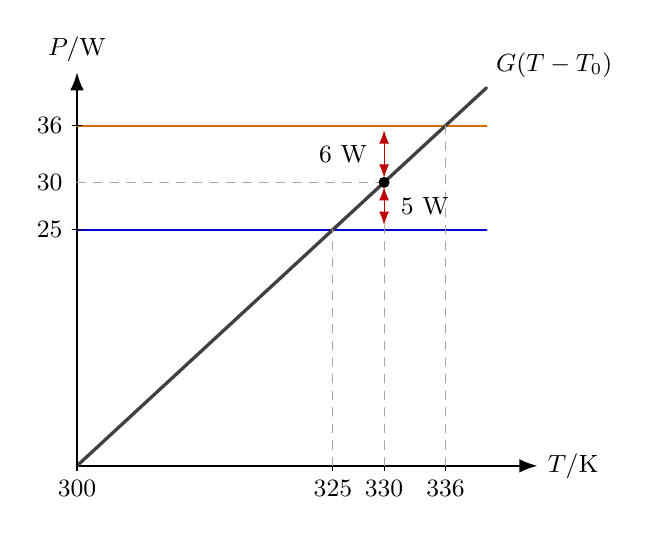
\begin{tikzpicture}
 \draw[->,thick](0,0)--(5.85,0)node[right]{$T/\mathrm K$};
 \draw[->,thick](0,0)--(0,5.0)node[above]{$P/\mathrm W$};
 \draw[blue!80!black,thick](0,3.00)--(5.2,3.00);
 \draw[orange!85!black,thick](0,4.32)--(5.2,4.32);
 \draw[very thick,black!75](0,0)--(5.2,4.80);
 \node[above right]at(5.20,4.80){$G(T-T_0)$};
 \foreach \x/\lab in {0/300,3.25/325,3.9/330,4.68/336}{
  \draw(\x,.06)--(\x,-.06)node[below]{$\lab$};
 }
 \draw(.06,3.0)--(-.06,3.0)node[left]{$25$};
 \draw(.06,4.32)--(-.06,4.32)node[left]{$36$};
 \draw[guide](3.25,0)--(3.25,3.00);
 \draw[guide](4.68,0)--(4.68,4.32);
 \draw[guide](3.9,0)--(3.9,3.60);
 \draw[guide](0,3.60)--(3.9,3.60);
 \node[left]at(-.06,3.60){$30$};
 \fill(3.9,3.60)circle(2pt);
 \draw[<->,thin,red!75!black](3.9,3.66)--(3.9,4.26);
 \node[left]at(3.81,3.96){$6\ \mathrm W$};
 \draw[<->,thin,red!75!black](3.9,3.06)--(3.9,3.54);
 \node[right]at(3.99,3.30){$5\ \mathrm W$};
\end{tikzpicture}

% 6: Plateau--control--plateau; x is rod movement, not piston movement.
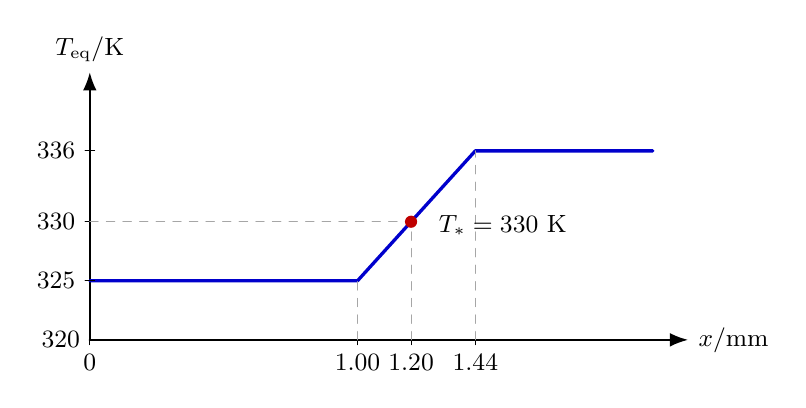
\begin{tikzpicture}
 \draw[->,thick](0,0)--(7.60,0)node[right]{$x/\mathrm{mm}$};
 \draw[->,thick](0,0)--(0,3.40)node[above]{$T_{\rm eq}/\mathrm K$};
 \draw[very thick,blue!80!black](0,.75)--(3.4,.75)--(4.896,2.4)--(7.15,2.4);
 \foreach \y/\lab in {.75/325,1.5/330,2.4/336}{
  \draw(.06,\y)--(-.06,\y)node[left]{$\lab$};
 }
 \node[left]at(0,0){$320$};
 \draw(0,.06)--(0,-.06)node[below]{$0$};
 \foreach \x/\lab in {3.4/1.00,4.08/1.20,4.896/1.44}{
  \draw(\x,.06)--(\x,-.06)node[below]{$\lab$};
 }
 \draw[guide](3.4,0)--(3.4,.75);
 \draw[guide](4.896,0)--(4.896,2.4);
 \draw[guide](4.08,0)--(4.08,1.5);
 \draw[guide](0,1.5)--(4.08,1.5);
 \fill[red!75!black](4.08,1.5)circle(2.2pt);
 \node[right]at(4.31,1.45){$T_\ast=330\ \mathrm K$};
\end{tikzpicture}
\end{document}
